% Paso 5 c) y d) (Luis).
\subsection{Perspectivas de contexto}
% Paso 5 c): las ocho perspectivas de contexto de Pohl aplicadas al PFC.
% Para cada una: 3 preguntas clave y 2 requisitos o restricciones que salen de ella.

\subsection{Mapa conceptual integrador}
% Paso 5 d): mapa en draw.io con los cuatro temas de la unidad y mínimo 3 vínculos cruzados.
% Exportarlo como PNG o PDF a la carpeta figuras/ y quitar el comentario de las líneas de abajo.
% \begin{figure}[h]
%   \centering
%   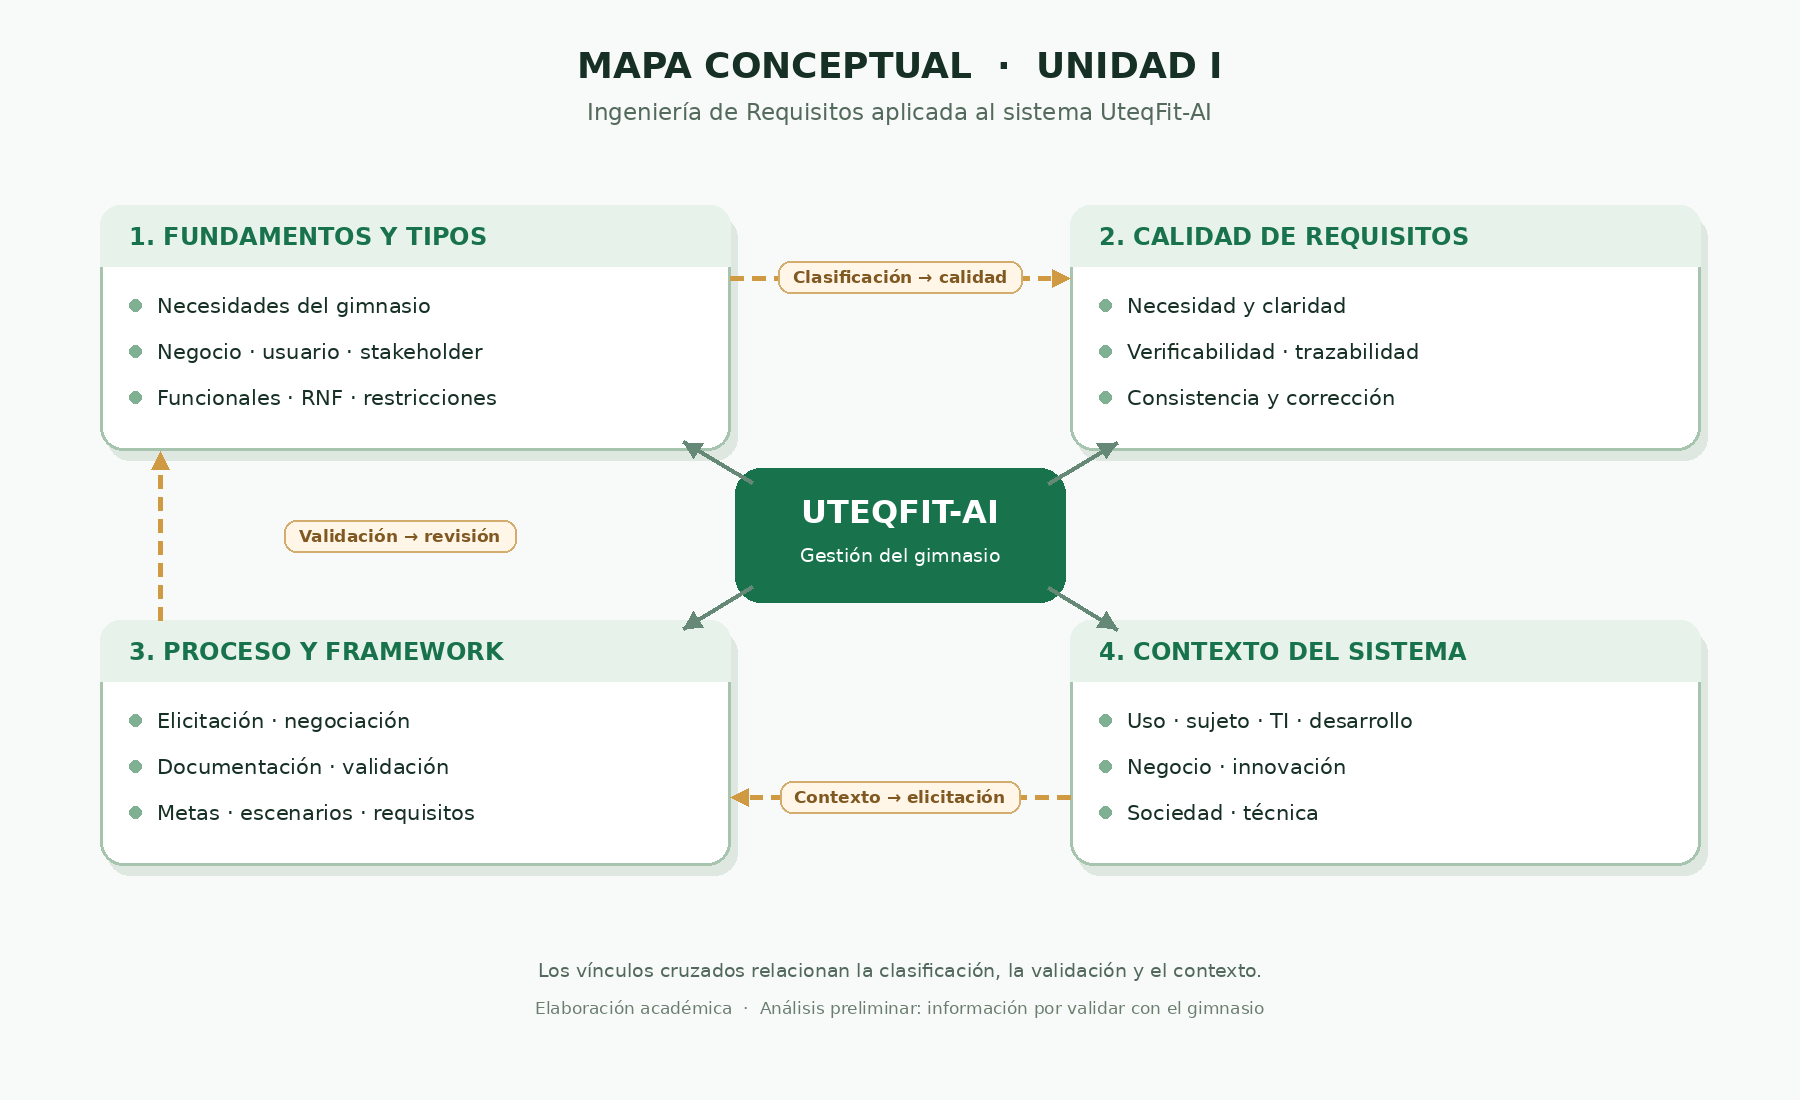
\includegraphics[width=\textwidth]{figuras/mapa_conceptual.png}
%   \caption{Mapa conceptual integrador de la unidad 1}
%   \label{fig:mapa}
% \end{figure}
